\PassOptionsToPackage{hyperfootnotes=false}{hyperref}
\documentclass[a4paper,fleqn]{cas-sc}

\usepackage[authoryear,longnamesfirst]{natbib}

\graphicspath{{figures/}}

\begin{document}
\let\WriteBookmarks\relax
\def\floatpagepagefraction{1}
\def\textpagefraction{.001}

\emergencystretch=3em

% Short title
\shorttitle{Hypothetica}

% Short author
\shortauthors{M. Karakaya et~al.}

% Main title
\title[mode=title]{Hypothetica: A Multi-Agent Framework for
  Literature-Based Novelty Assessment of Research Ideas}
\tnotemark[1]

% Title footnote
\tnotetext[1]{This study was carried out as part of the SENG~491 --
CMPE~491 -- SENG~492 -- CMPE~492 Senior Project I -- Senior Project II
courses, under the supervision of Dr.\ Murat Karakaya at TED University.}

% First author
\author[1]{Harun H\"{u}dai Tan}
\ead{harunhudai.tan@tedu.edu.tr}
\credit{Conceptualization, Methodology, Software, Writing -- Original Draft}

\affiliation[1]{organization={Department of Software Engineering, Ted University},
               addressline={Ziya G\"{o}kalp Caddesi No: 48, Kolej, \c{C}ankaya},
               city={Ankara},
               postcode={06420},
               country={T\"{u}rkiye}}

% Second author
\author[1]{Baran Erol}
\ead{baran.erol@tedu.edu.tr}
\credit{Software, Validation}

% Third author
\author[1]{Ahmet Alp Malko\c{c}}
\ead{ahmetalp.malkoc@tedu.edu.tr}
\credit{Software, Validation}

% Fourth author
\author[2]{Kutay Becerir}
\ead{kutay.becerir@tedu.edu.tr}
\credit{Software, Validation}

\affiliation[2]{organization={Department of Computer Engineering, Ted University},
               addressline={Ziya G\"{o}kalp Caddesi No: 48, Kolej, \c{C}ankaya},
               city={Ankara},
               postcode={06420},
               country={T\"{u}rkiye}}

% Fifth author
\author[1]{Murat Karakaya}
\cormark[1]
\ead{murat.karakaya@tedu.edu.tr}
\credit{Supervision, Writing -- Review \& Editing}

% Corresponding author text
\cortext[1]{Corresponding author: murat.karakaya@tedu.edu.tr}

\begin{abstract}
Researchers often need to spend a lot of time manually reviewing
prior studies to confirm that a proposed project does not repeat
existing work, and this process can be slow.
This paper introduces Hypothetica, an AI-powered system that evaluates
the originality of proposed research ideas by comparing them with
prior art from academic literature, patents, and public code
repositories. The system uses a multi-agent architecture based on large
language models, combined with retrieval-augmented generation (RAG), to
support explainable assessments of originality. The system retrieves
candidate evidence from OpenAlex, arXiv, Google Patents, and GitHub,
then reviews the material across four dimensions: problem similarity,
method similarity, domain similarity, and contribution similarity.
Hypothetica produces a numerical originality score and detailed
reports with evidence-based feedback, mapping sentences in the user's
research idea to related passages in the retrieved sources. The
system's performance was assessed on a 135-case benchmark spanning
three evidence corpora: OpenAlex, Google Patents, and GitHub. In this
evaluation, Hypothetica achieved 75.6\% mean classification accuracy,
with all misclassifications occurring only between adjacent originality
classes. These results indicate that the approach provides a coherent
originality signal across different evidence sources and can help
researchers refine their ideas using clear, practical feedback before
they begin their research.
\end{abstract}

\begin{highlights}
\item Hypothetica assesses research idea originality using a multi-agent RAG pipeline.
\item The system compares ideas against academic literature, patents, and public code repositories.
\item A 135-case benchmark shows 75.6\% mean accuracy with only adjacent-class errors.
\end{highlights}

\begin{keywords}
large language models \sep multi-agent systems \sep research originality \sep retrieval-augmented generation
\end{keywords}

\maketitle

\section{Introduction}
\label{sec:introduction}

In order to prevent duplicating work and wasting resources, researchers must verify their hypotheses against existing literature. As the volume of scientific publications has grown, this verification has become substantially harder. As of December 2025, arXiv lists 2,911,812 submissions and receives more than 26,000 new paper submissions per month \citep{arxivStats}. Since its launch in 1991, arXiv has expanded to a scale at which researchers often struggle to read and assess all relevant work before starting a new study. The rapid growth of academic publishing has produced a clear need for tools that can assess the originality of research consistently and reliably. Manual literature reviews are time consuming and frequently left incomplete, and they rarely identify precise similarities between new concepts and earlier work. They also tend to overlook prior art that lives outside academic preprints, such as patent records and public code repositories, which often document the same ideas as research papers but in different forms.

The rapid development of Large Language Models (LLMs) has made automated validation of research ideas tractable, especially for natural language understanding and information retrieval tasks. Recent work shows that LLMs are already used effectively in literature review \citep{eger2025}. However, single LLMs do not have the analytical depth required to assess the novelty of a research idea reliably. Single-prompt models perform basic comparisons and remain vulnerable to hallucination, in contrast to autonomous multi-agent systems that decompose the task across specialised roles \citep{zheng2025}. Standard retrieval systems return related papers but do not produce a structured judgement on novelty. To address this gap, our approach builds an autonomous environment in which multiple agents perform retrieval, paper-by-paper scrutiny, and global synthesis. A growing body of recent work has begun to frame literature-grounded research idea novelty as a distinct task, moving beyond simple semantic similarity toward retrieval-backed and more explainable assessment workflows \citep{shahid2025,lin2025schnovel,scholareval,rinobench,opennovelty,dasilva2025graphmind}, and beyond pure novelty checking toward broader research-assistant systems for the scientific lifecycle \citep{eger2025survey,wang2024scimon,si2024llmideas,lu2024aiscientist,baek2024researchagent}.

This study presents Hypothetica \citep{hypotheticaGitHub}, an AI-driven research validation system that evaluates the originality of a proposed research concept against multiple sources of prior art. Rather than restricting itself to a single repository, Hypothetica retrieves evidence through a pluggable adapter layer that unifies scholarly works from OpenAlex \citep{openalexDocs,priem2022openalex} and arXiv \citep{arxivAPI}, patent records from Google Patents, and open-source repositories from GitHub under a single originality-scoring pipeline. The system generates originality reports using a multi-agent architecture driven by Google Gemini \citep{geminiAPI} and a Retrieval Augmented Generation (RAG) architecture \citep{lewis2020rag,gao2024ragsurvey}, so researchers can make informed decisions about their concept on the basis of evidence drawn from across the academic, industrial, and software ecosystems.

The analysis pipeline is divided into two layers and assesses each research concept along four dimensions: novelty of the technical problem, methodological innovation, overlap in the application domain, and similarity of the claimed contribution. It integrates RAG with originality scoring, semantic chunking, and dense vector retrieval based on E5 embeddings \citep{wang2022e5} and Chroma \citep{chroma}, followed by cross-encoder reranking \citep{nogueira2019monobert} before any candidate reaches the scoring layer. Before retrieval, a conversational interview agent elicits missing details about the idea over a short multi-round dialogue, and a reality-check agent runs in parallel to flag whether the proposed concept already exists as a known product or system, independently of what the corpus returns. For source types where document-level granularity is more appropriate than passage-level retrieval, such as GitHub README files, the same scoring layer consumes the document as a whole rather than as embedded chunks. In addition to a numerical originality score, the system features a report generation component that links specific sentences in the user's research idea to the relevant sections of the retrieved sources considered in the report.

The primary contributions of this study are as follows. First, we introduce Hypothetica, an automated system designed to transform manual originality assessment into an LLM-based computational pipeline. Second, we propose a specialised multi-agent architecture that improves assessment quality compared to single-prompt baselines by assigning dedicated agents to specific roles, including a conversational interview agent for clarifying the idea, a reality-check agent for surfacing already-existing products, query-variance and relevance-filtering agents for retrieval, and per-paper Layer~1 and global Layer~2 agents for scoring and aggregation. Third, we design a pluggable evidence-adapter layer that lets the same scoring pipeline reason over heterogeneous prior art (academic works from OpenAlex and arXiv, patent records from Google Patents, and open-source repositories from GitHub) without changes to the scoring agents themselves. Fourth, instead of merely producing an overall evaluation score, our system shows exactly which parts of the user's idea match existing work by linking sentences to specific passages in the retrieved sources.

\section{Related Work}
\label{sec:related_work}

\subsection{Plagiarism Detection and Novelty Assessment}

Assessing novelty is often confused with plagiarism checking, but the two tasks differ substantially in goal and method. Commercial tools such as Turnitin Similarity \citep{turnitin} and iThenticate \citep{ithenticate} measure surface text overlap and flag missing or inconsistent citations and attributions. They do not assess novelty at the level of ideas, methodology, or contribution; their outputs function as similarity indicators rather than conclusions about conceptual novelty.

When evaluating a research idea, conceptual overlap and textual overlap must be distinguished. Two papers can describe the same underlying idea with little shared wording, while a genuinely new study may still need to reuse common terms such as standard metrics and widely accepted definitions. Similarity reports therefore support academic integrity checks but do not directly answer whether an underlying idea is original.

\subsection{Literature Search and Discovery Tools}

A wide range of tools has emerged to support finding relevant literature and mapping citations, which is a separate goal from quantitative novelty scoring. Semantic Scholar \citep{semanticScholar} applies machine-learning methods to support literature search and the exploration of publication metadata. Connected Papers \citep{connectedPapers} and Research Rabbit \citep{researchRabbit} use graph-based methods to map relationships among related studies. Elicit \citep{elicit} reduces the manual effort in systematic literature reviews by automating parts of screening and data extraction. Scite \citep{scite} uses Smart Citations to label cited works as supporting, contrasting, or mentioning, helping readers judge the strength and direction of evidence. While these systems improve screening and triage, they typically do not provide a clear, rule-based originality score with sentence-level tracking that can be checked against a specific user hypothesis.

\subsection{Literature-Grounded Idea Novelty Systems}

Relying solely on an LLM to judge novelty is risky, because the model can present conclusions confidently even when those claims cannot be checked against verifiable evidence. Retrieval-augmented generation (RAG) is a widely used remedy: it combines text generation with retrieval from an external corpus to improve factual accuracy and to record the sources used \citep{lewis2020rag,gao2024ragsurvey}. The broader notion of novelty itself has earlier roots in information retrieval, where the TREC Novelty Track \citep{harman2002trec} formalised novelty as the sentence-level identification of new information in a document stream. Although the target object differs from scientific idea novelty, the conceptual move from document-level relevance to sentence-level novelty remains influential and motivates the sentence-level overlap reports produced by Hypothetica.

Several recent systems target literature-grounded idea novelty more directly. \citet{shahid2025} propose the Idea Novelty Checker, a retrieve-then-rerank pipeline that evaluates the novelty of a scientific idea using retrieved literature, expert-annotated examples, and a facet-based operational definition of novelty. The output is binary, novel or not novel, and the judgement depends on whether the idea differs from prior work in core facets such as purpose, mechanism, or evaluation. The work demonstrates that novelty assessment quality depends strongly on retrieval quality and on having a clearer operational notion of novelty than generic semantic similarity. In contrast, Hypothetica uses a multi-agent design with separate stages for retrieval, paper-by-paper analysis, and synthesis, draws candidates from multiple corpora through a unified adapter layer rather than from a single literature index, and replaces a binary verdict with a four-dimensional Likert-based assessment whose criterion weights are calibrated against an arXiv benchmark.

\citet{lin2025schnovel} take a complementary, benchmark-first angle. They construct SchNovel, a 15,000-pair benchmark of academic papers across six fields, and propose RAG-Novelty, a retrieval-augmented pipeline that assigns a 0-to-10 novelty score to a query paper after comparing it against top-K retrieved prior work. Their ground truth is operationalised by treating the newer paper in each pair as the more novel one, which scales well but is acknowledged as a debatable proxy across domains. Hypothetica differs in three ways. It scores user-supplied research ideas rather than already-published papers, it replaces a single 0-to-10 axis with four independently-scored criteria with empirically calibrated weights, and it grounds each score in sentence-level evidence rather than abstract-only retrieval.

A second direction broadens the task beyond binary novelty judgement. ScholarEval \citep{scholareval} evaluates research ideas on two criteria, soundness and contribution, using a multi-stage pipeline that retrieves method-level and dimension-level evidence from literature before synthesising strengths, weaknesses, contradictions, and suggestions. ScholarEval moves toward richer reviewer-style feedback rather than a single novelty verdict. Compared to ScholarEval, Hypothetica is narrower in scope, focused specifically on originality assessment, but it similarly emphasises structured, evidence-grounded analysis instead of a single opaque judgement. Hypothetica also broadens the notion of relevant literature to include patent records and public code repositories alongside academic works.

RINoBench \citep{rinobench} formalises research idea novelty assessment as the joint prediction of a rubric-based 1-to-5 novelty score and a grounded textual justification. It is benchmark-oriented rather than system-oriented: it argues that novelty-assessment systems should be evaluated not only on the score they assign, but also on whether their explanations align with grounded human reasoning. This is particularly relevant for systems such as Hypothetica, because plausible reasoning and accurate scoring do not always coincide.

OpenNovelty \citep{opennovelty} focuses on verifiable scholarly novelty assessment. It extracts a paper's core task and claimed contributions, retrieves prior work through expanded semantic queries, organises related work into a hierarchical taxonomy, and performs claim-level comparisons against retrieved papers. Refutation-style judgements are retained only when supported by verified evidence quotes from the source texts. This evidence-bound design is consistent with the broader literature on scientific claim verification, where systems trained on benchmarks such as SciFact \citep{wadden2020scifact} learn to retrieve and rationalise sentence-level evidence for or against a claim before issuing a verdict. Compared to Hypothetica, OpenNovelty is more claim-refutation-oriented and more centred on evidence verification and taxonomy construction, whereas Hypothetica is more directly focused on user-facing originality analysis through four-dimensional scoring and sentence-level overlap mapping over a heterogeneous evidence base that combines academic works, patents, and code.

\citet{dasilva2025graphmind} introduce GraphMind, an interactive novelty-assessment tool that combines arXiv and Semantic Scholar APIs with LLM-based extraction to produce structured macro-level (paper graph) and micro-level (claim and section) views of related work, with explicit emphasis on traceability through an information-retrieval module that returns supporting and contrasting evidence. GraphMind is the closest existing tool to Hypothetica in terms of user-facing scope and evidence-traceability emphasis. The two systems differ in evidence base, with GraphMind drawing only from academic literature whereas Hypothetica retrieves additionally from patents and code through its adapter layer; in scoring layer, with GraphMind producing a qualitative report whereas Hypothetica produces a four-criterion Likert-based numerical score with categorical guardrails; and in interaction style, with GraphMind providing an exploratory web tool whereas Hypothetica runs an end-to-end pipeline that begins with a conversational interview to clarify the proposed idea before retrieval.

Beyond pure novelty checking, recent work has explored broader research-assistant systems built on LLM agents. \citet{eger2025survey} survey this fast-moving ecosystem across the full scientific lifecycle, including search, ideation, experimentation, content generation, and evaluation, providing a useful map for situating originality-assessment work among related AI-for-science tools. Within that ecosystem, SciMON \citep{wang2024scimon} explicitly optimises for novelty during scientific hypothesis generation by retrieving and contrasting against prior literature, reinforcing the view that novelty must be measured against retrieved evidence rather than assumed from the model alone. \citet{si2024llmideas} conduct a large-scale human study on whether LLMs can generate novel research ideas, finding that LLM-produced ideas are sometimes perceived as more novel than human-produced ideas but weaker in feasibility, which underscores the importance of grounding any novelty signal in retrieved evidence. ResearchAgent \citep{baek2024researchagent} iteratively refines research ideas using literature-grounded LLM agents, while The AI Scientist \citep{lu2024aiscientist} proposes an end-to-end pipeline for automated open-ended scientific discovery covering idea generation, experiment design, and write-up. These systems share Hypothetica's reliance on coordinated LLM agents but pursue idea generation, refinement, or experimentation rather than originality assessment of a user-supplied idea.

\subsection{Dense Retrieval and Cross-Encoder Reranking}

Established information-retrieval practice combines sparse lexical matching, dense embedding retrieval, and a learned reranker. Sparse methods such as BM25 \citep{robertson2009bm25} remain strong baselines for short queries with rare terms, and the BEIR benchmark \citep{thakur2021beir} shows that dense retrievers do not uniformly dominate sparse ones in zero-shot settings, which motivates the use of learned rerankers on top of dense first-stage retrieval. Dense retrievers project queries and documents into a shared vector space; the E5 family of contrastively pre-trained encoders \citep{wang2022e5} is one such family, used in this work. Cross-encoder rerankers, such as the BERT-based passage re-ranker introduced by \citet{nogueira2019monobert}, jointly encode query and document and produce relevance scores that are usually more accurate than pure bi-encoder similarity, at the cost of higher inference time.

Hypothetica adopts the standard two-stage design. It uses E5 embeddings stored in Chroma \citep{chroma} for first-stage retrieval, then applies cross-encoder reranking over a top-k candidate set before any document is forwarded to the scoring layer. For the OpenAlex adapter, an additional pre-ranking step weighs first-stage relevance, citation count, and recency before the embedding stage, because the unfiltered OpenAlex result set is much larger than the arXiv result set and benefits from a coarse pre-filter before any expensive computation.

\subsection{LLM-as-Judge and Rubric-Based Evaluation}

Hypothetica's per-paper scoring layer (Layer~1) follows the LLM-as-judge paradigm, in which a language model rates a target item against a set of criteria. G-Eval \citep{liu2023geval} proposed using GPT-4 with chain-of-thought prompting and form-filling to evaluate generated text against task-specific rubrics, reporting better correlation with human judgements than earlier reference-based metrics. MT-Bench and Chatbot Arena \citep{zheng2023mtbench} systematically studied LLM-as-judge agreement with human ratings on multi-turn benchmarks and identified well-known biases, including position bias and verbosity bias. Prometheus \citep{kim2024prometheus} showed that fine-grained, rubric-based evaluation does not necessarily require a frontier closed model: an open model trained on rubric-supervised data can match GPT-4 quality on many evaluation tasks. Closer to our setting, \citet{liang2024llmfeedback} conducted a large-scale empirical analysis of LLM-generated feedback on research papers across multiple journals and a major machine-learning conference, reporting that LLM feedback overlaps substantially with human reviewer comments while tending to be less specific and more uniform than human reviews. That study targets free-form reviewer-style feedback rather than per-criterion originality scoring, but it confirms that LLMs can produce useful, partially human-aligned judgements over academic text when prompted carefully.

These works inform two specific choices in Hypothetica. Each criterion is scored independently with its own Likert rubric in order to reduce halo effects, and the criterion weights used in Layer~2 are not uniform but calibrated empirically against a labelled arXiv benchmark, so that criteria with stronger discriminative power dominate the global score. Categorical guardrails additionally constrain the global score whenever any single criterion reaches its top Likert level, which mitigates the verbosity and overconfidence biases that pure averaging would otherwise allow.

\subsection{Multi-Agent LLM Architectures}

Agentic decomposition has been adopted to make complex LLM pipelines more structured and easier to audit. Surveys of LLM-based multi-agent systems describe common architectures and recurring issues such as coordination, verification, and reliability \citep{guo2024multiagent,zheng2025}. Frameworks such as AutoGen \citep{wu2023autogen} formalise multi-agent coordination among LLM agents through structured message passing, and broader surveys of retrieval-augmented generation \citep{gao2024ragsurvey} argue for similarly modular pipelines that separate retrieval, generation, and verification.

Hypothetica follows this trend by dividing the pipeline into specialised agents: a conversational interview agent that clarifies the proposed idea over a short multi-round dialogue, a reality-check agent that runs in parallel to flag potentially already-existing products, a query-variant agent that generates adapter-aware search queries, a relevant-paper-selector agent that filters reranked candidates, a Layer~1 per-paper analysis agent that scores the four originality criteria with per-criterion Likert rubrics, and a Layer~2 aggregation step that combines per-paper scores into a global originality score with categorical guardrails. For GitHub-based evidence, additional repository-relevance and synthesis agents replace the chunk-based retrieval flow. The pipeline requires structured outputs at every stage so that downstream scoring stays adequately deterministic and the user interface can provide clear explanations for each score.

\subsection{Beyond Academic Literature: Patents and Code as Prior Art}

Academic preprints are not the only form of prior art relevant to research originality. Industrial novelty is documented in patent records, and working systems are documented in public code repositories. Both have received attention from the information-retrieval community.

Patent prior-art retrieval is a long-standing task with its own conventions and benchmarks. \citet{krestel2021patents} survey deep-learning approaches to patent analysis, including classification, retrieval, and similarity assessment, and emphasise that patents differ from academic abstracts in length, terminology, and legal-style framing. These differences justify including patents as a first-class evidence source in originality assessment, because a research idea that is already disclosed in a patent is not novel even if no academic paper has yet been published on it.

Public code repositories provide a third channel of prior art that academic-only systems miss. From a novelty-assessment standpoint, the existence of a maintained repository that implements the proposed idea is a direct, often stronger signal than a paper that only describes it. Hypothetica embeds repository README files as natural-language documents using the same E5 encoder used for paper abstracts, rather than relying on code-specific embeddings, on the grounds that READMEs are written in prose and the originality decision is made by the LLM scoring agent rather than by the embedding similarity alone.

Hypothetica integrates these two evidence types alongside academic works. Patents are searched through Google Patents \citep{serpapi}, and repositories are searched on GitHub \citep{githubAPI}. Both adapters share the same pipeline interface as the OpenAlex and arXiv adapters, so the same scoring agents reason uniformly over heterogeneous sources without source-specific adjustments.

\subsection{Positioning of Hypothetica}

Hypothetica uses an evidence-first method aligned with retrieval-augmented generation. Instead of returning a single opaque score, it reports sentence-level flags and points to matching excerpts in the retrieved sources, so users can check the evidence behind each flagged passage. The system is therefore useful not only for producing a final score but also for showing where overlap occurs and why. While the initial Hypothetica prototype drew its corpus solely from arXiv using the official arXiv API \citep{arxivAPI}, the current system retrieves evidence through a pluggable adapter layer that integrates OpenAlex \citep{openalexDocs,priem2022openalex} for broad cross-disciplinary scholarly works, arXiv \citep{arxivAPI} for preprints in computer science and machine learning, Google Patents for industrial prior art, and GitHub repositories for working open-source implementations whose existence often invalidates novelty claims even when no paper has yet been published. The same interface can accommodate additional sources such as the Semantic Scholar API \citep{semanticScholarAPI} without changes to the scoring agents. In this respect, Hypothetica aligns with the recent movement toward grounded, multi-source, and inspectable originality analysis, while remaining distinct from generic similarity tools and from purely parametric LLM judgements.

\section{Methodology}
\label{sec:methodology}

Hypothetica is designed as a multi-stage originality assessment pipeline. Given a natural language research idea and a selected evidence source, the method produces an enriched idea representation, retrieves candidate prior work, selects a small set of highly relevant resources, parses their content, and computes an originality score for the submitted idea. The final assessment reports the overall originality score, similarity scores for four originality criteria, and the evidence passages that explain the strongest similarities with prior work.

Originality assessment requires more than surface-level text matching. Two ideas may describe the same technical contribution using different terminology, while a genuinely novel idea may still share domain vocabulary with existing work. Hypothetica therefore combines semantic retrieval, cross-encoder reranking, and large language model reasoning to support concept-level comparison between the submitted idea and prior work. The pipeline is organized into phases with explicit data boundaries so that each step, from retrieval to final score computation, can be analyzed independently.

\subsection{System Overview}

\paperfigureblock[0.88\linewidth][0.36\textheight]{"Hypothetica Flowchart/GeneralOverview.png"}{System Overview Diagram.}{fig:overview}

Hypothetica is structured as a multi-phase pipeline that takes a natural language research idea as input and produces a structured originality assessment as output, as shown in Fig.~\ref{fig:overview}. The pipeline begins with a User Interaction Phase that turns the raw submission into an enriched, well-defined idea description, and continues through a Retrieval Phase that gathers candidate prior art from the user's selected evidence source. A Candidate Selection Phase then narrows this pool down to a small, high-quality shortlist through a combination of vector-based filtering, cross-encoder reranking, and an LLM-based selection step. Once the shortlist is fixed, the Parsing Phase converts each selected resource into structured, searchable text and indexes it in a vector store. The two scoring phases that follow are where the originality verdict is produced: the Candidate Originality Scoring phase analyzes each shortlisted resource independently against the user's idea and produces per-criterion similarity scores together with sentence-level similarity evidence, and the Idea Originality Scoring phase aggregates these per-resource results into a single global originality score, a labeled breakdown across the four originality criteria, and a sentence-level annotation of the user's idea. The final output includes the global originality score, criterion-level similarity values, sentence-level originality labels, and evidence passages that explain the strongest similarity judgments.

The phases communicate through structured data passed from one stage to the next, and the boundaries between them are deliberate: each phase has a single, well-defined responsibility, which makes the pipeline easier to extend with new evidence sources, new scoring criteria, or reporting formats without disturbing the rest of the system. The pipeline exposes parameters for retrieval depth, reranking depth, final resource selection, and final score computation. The default values for these parameters are described in Section~\ref{sec:testing} and summarized in Table~\ref{tab:params}. The remainder of this section describes each phase in detail.

\subsection{User Interaction Phase}

\paperfigureblock[0.48\linewidth][0.50\textheight]{"Hypothetica Flowchart/User-Interaction-Phase.png"}{User Interaction Diagram.}{fig:user_interaction}

The pipeline begins with the User Interaction Phase, which transforms a raw user submission into a structured input that the rest of the system can operate on. As shown in Fig.~\ref{fig:user_interaction}, this phase takes a User Request Payload and produces an Enriched Idea that is passed forward to the Retrieval Phase.

The first step is an Adapter Availability Check. Before any analysis begins, the system verifies that the adapter chosen by the user, such as OpenAlex, Google Patents, or GitHub, is configured and accessible. If the selected adapter is unavailable, the request is rejected. This early validation prevents wasted computation and gives the user immediate feedback when an evidence source cannot be reached.

Once the adapter is confirmed to be available, the Follow-Up Questions step is triggered. A dedicated agent reads the user's research idea and generates three clarifying questions. These questions are designed to cover aspects such as the specific research problem being addressed, the proposed method or approach, and the parts of the idea the user considers novel. The purpose of this step is to surface information that researchers often leave implicit in a short idea description but that is important for targeted retrieval and scoring. Without this clarification, vague ideas tend to lead to less focused retrieval and shallower per-paper analysis later in the pipeline.

The user's responses to these questions are then passed to the Idea Enrichment step. Here, the original idea and the question-answer pairs are combined into a single, structured text block that preserves both the user's initial idea and the additional details provided through the clarifications. This combined text is the Enriched Idea that drives later stages of the pipeline. From this point, retrieval queries, candidate selection, per-paper scoring, and global originality scoring all operate on the enriched description rather than on the raw input.

\subsection{Retrieval Phase}

\paperfigureblock[0.52\linewidth][0.58\textheight]{"Hypothetica Flowchart/Retrieval-Phase.png"}{Retrieval Phase Diagram.}{fig:retrieval}

Once the Enriched Idea Context is produced, the pipeline enters the Retrieval Phase, which is responsible for retrieving a large pool of candidate resources from the selected adapter. As shown in Fig.~\ref{fig:retrieval}, this phase takes the Retrieval Input consisting of the Enriched Idea and the Selected Adapter chosen earlier by the user and outputs N Unique Candidates that are forwarded to the Candidate Selection Phase. The main challenge at this stage is balancing recall and precision. If the search is too narrow, it risks missing important prior work altogether. On the other hand, if it is too broad, it brings back a large number of documents, many of which are not relevant. For this reason, the Retrieval Phase is designed to focus more on recall, while precision is improved later during the filtering steps.

The process starts with Query Variant Generation. Instead of relying on a single query based on the user's idea, a Query Variant Agent produces a structured set of complementary search queries. For general scholarly and patent retrieval, the query set contains a raw query that condenses the core idea, two academic reformulations that separately emphasize the method and the application domain, and a synonym query that captures abbreviations and alternative terms. This structure is intended to support broader recall by covering both natural-language descriptions and the terminology that is likely to appear in titles, abstracts, or patent descriptions.

The query strategy is adapter-aware. For OpenAlex, which performs relevance-ranked full-text search over a broad scholarly index, the agent produces five variants: a raw query, a method-focused academic query, a domain-focused academic query, a synonym query, and a concept-level query that targets related subfields, benchmark names, or survey-level terminology. For GitHub, the agent instead produces four implementation-focused queries built around rare technical terms, framework names, and repository-language expressions, while avoiding generic standalone terms such as ``agent'', ``LLM'', or ``tool''. If query generation fails, the pipeline falls back to a single raw query based on the enriched idea, so retrieval can still proceed.

The Variant Queries List is then sent, one query at a time, to the Adapter Search step. The selected adapter -- OpenAlex, Google Patents, or GitHub -- is invoked through a unified adapter interface that hides the differences between the underlying source services. Each adapter is responsible for issuing the query to its corresponding service, parsing the source-specific response, and converting the raw results into a standardized Resource representation that the rest of the pipeline can operate on. For each query variant, the adapter retrieves candidates up to a configurable retrieval-depth parameter. Operating through this adapter abstraction supports adding new evidence sources without changing the rest of the pipeline.

After all the variant searches finish, the Deduplication step merges their results into a single pool. Since each variant describes the same idea from a slightly different angle, the same resource often shows up in more than one result set, and the system needs to make sure it is only carried forward once. To handle this, deduplication relies on stable identifiers like the OpenAlex Work ID, the patent ID, or the repository's full name, and falls back to DOI when one is available. Anything that survives this step is given a fresh internal ID so the rest of the pipeline can refer to it consistently.

The final output of the Retrieval Phase is a set of N Unique Candidates, where N typically ranges from a few dozen to several hundred depending on the chosen adapter, the retrieval-depth setting, and the number of duplicates removed. N is therefore a run-level output rather than a separate fixed parameter; the default retrieval-depth value is described in the experimental setup and summarized in Table~\ref{tab:params}. This pool is intentionally larger than what would be analyzed in detail, since the goal of this phase is to maximize the chance that any prior work with meaningful similarity to the user's idea is included. Reducing this pool to a small, high-quality set is the responsibility of the next stage, the Candidate Selection Phase.

\subsection{Candidate Selection Phase}

\paperfigureblock[0.52\linewidth][0.58\textheight]{"Hypothetica Flowchart/Candidate-Selection-Phase.png"}{Candidate Selection Diagram.}{fig:candidate_selection}

The Candidate Selection Phase is responsible for tightening this pool down to a small, high-quality set of resources that will be used for detailed analysis. As shown in Fig.~\ref{fig:candidate_selection}, the input to this phase is the Candidate Selection Input, consisting of N Candidates from the Retrieval Phase together with the Enriched Idea, and the output is a fixed number of highly relevant resources that will be passed to the Parsing Phase. The default value is described in the experimental setup and summarized in Table~\ref{tab:params}. The phase is structured as a three-step process that combines vector-based filtering, a more precise but heavier reranking step, and finally a Large Language Model for judgment.

The first stage is Embedding Generation. Each candidate's title and abstract or, in the case of code repositories, the repository description and available documentation are embedded into a dense vector representation using a pretrained text embedding model. Once embeddings are available, the Semantic Similarity Ranking step computes the cosine similarity between the Enriched Idea vector and each candidate vector, and keeps the most similar ones according to a configurable embedding-stage cutoff. This stage removes many low-relevance candidates: candidates that share keywords with the idea but are conceptually unrelated tend to fall away, while candidates that talk about the same underlying problem in different words tend to surface. At this stage the system keeps the candidate set wide rather than aggressive, because the goal is to feed a high-recall input into the more precise reranker.

The second stage is Cross Encoder Reranking. Unlike the embedding step, which encodes the query and each document independently and only compares them at the end, a cross encoder takes the query and a single document together and produces a similarity score in one pass. This usually provides a more precise relevance signal because the model can attend to the interaction between specific words in the query and specific words in the document, but it is also considerably more expensive, which is why it only runs on the top candidates produced by the embedding step. The output of this stage is a top-ranked shortlist whose size is configurable and passed to a language model for the final selection.

The final stage is the Relevance Selection Agent, which acts as an LLM-as-a-judge over the reranked shortlist. Its input is the Enriched Idea and the top-ranked candidates that survived the embedding and cross-encoder stages. For scholarly or patent candidates, the agent receives the title, abstract or description, source metadata, and the available rerank or similarity score; for code repositories, it receives the repository title, description, available documentation content, repository metadata, and the available score. These scores are treated as supporting signals rather than as the final decision rule. The agent is instructed to select the resources that are most useful for a deeper originality analysis by prioritizing conceptual alignment, direct methodological relevance, similar problem framing, and evidence that helps compare the user's proposed approach with prior work. For repository evidence, the criteria are adapted toward implementation quality, feature completeness, code maturity, and direct applicability to the user's idea. The output is a structured list of selected resource identifiers with short selection reasons; if the LLM selection fails or returns no usable identifiers, the pipeline falls back to the top candidates from the cross-encoder ranking.

The output of the Candidate Selection Phase is the final resource list that will be analyzed in detail in the rest of the pipeline. By the time a resource reaches this point, it has passed three filters -- vector similarity, cross-encoder reranking, and language model judgment -- which together provide a stronger relevance signal than any single retrieval step could offer on its own.

\subsection{Parsing Phase}

\paperfigureblock[0.56\linewidth][0.58\textheight]{"Hypothetica Flowchart/Parsing-Phase.png"}{Parsing Diagram.}{fig:parsing}

Before any per-candidate analysis can take place, each of the selected resources needs to be turned into structured, searchable text. This is the responsibility of the Parsing Phase, shown in Fig.~\ref{fig:parsing}. The phase takes the Top-K Candidates produced by the Candidate Selection Phase and ends with an indexed vector store containing the text chunks of every candidate, ready for retrieval during the scoring phases.

The phase begins with Parallel Document Fetching. Each candidate's available full content is collected concurrently from its source. PDFs are retrieved for OpenAlex, the Google Patents API is queried directly for patent descriptions, and the README content already collected during retrieval is reused for GitHub repositories. The fetched content is then converted into a Markdown representation so that the rest of the pipeline can treat resources from different adapters in the same way.

Once a uniform document is available, the Extract Section Content step parses out the structural skeleton of each resource. Headings are identified and the text under each heading is associated with that heading as its section content. Sections that contribute little to originality assessment, such as references, acknowledgments, and patent-specific legal sections, are skipped at this stage so that they do not pollute the downstream representation.

The remaining steps are repeated for each candidate. The Document Chunking Processor splits each section into smaller chunks, with target sizes chosen to fit the context windows of both the embedding model and the language model. The Vector Store Ingestion step then embeds these chunks and stores them with their source metadata. The output of the Parsing Phase is an indexed vector store ready to support retrieval during the Candidate Originality Scoring and Idea Originality Scoring phases.

\subsection{Candidate Originality Scoring}

\paperfigureblock[0.72\linewidth][0.54\textheight]{"Hypothetica Flowchart/Candidate-Originality-Scoring-Phase-Layer-1.png"}{Candidate Originality Scoring Diagram.}{fig:candidate_scoring}

The Candidate Originality Scoring phase is where each candidate is independently compared against the user's idea to produce a structured similarity profile. As shown in Fig.~\ref{fig:candidate_scoring}, the input to this phase is the Enriched Idea together with the processed candidates and the indexed candidate text, and the output is a per-candidate Candidate Originality Scoring Result containing a similarity score, criteria-level scores, sentence-level analysis, matched sections, and a justification for each score. The phase loops over every candidate and treats each one as a separate scoring task, so that a highly similar resource remains visible in the later aggregation stage.

For each candidate, the system first builds a focused textual representation of the resource. The Extracted Fixed Sections step pulls out parts of the document that are generally useful for originality assessment, such as the abstract, introduction, and conclusion when they are available. In parallel, the Contextual RAG Retrieval step queries the vector store with the Enriched Idea and retrieves the chunks from the same candidate that are most semantically aligned with it. Combining a fixed structural skeleton with retrieval-driven context lets the language model see both the standard parts of the resource and the parts that specifically discuss similar problems or methods, without overwhelming the prompt with the entire document.

This combined context is then passed to two parallel evaluation tracks. The first track is the Multi-Criterion LLM Evaluation, which scores the candidate against the Enriched Idea on four originality dimensions: Problem Similarity, Method Similarity, Domain Similarity, and Contribution Similarity. Problem Similarity measures whether the candidate addresses the same research question or gap. Method Similarity measures whether it uses the same technical approach, architecture, or pipeline. Domain Similarity measures whether it operates in the same application area, task setting, data type, or target system. Contribution Similarity measures whether the candidate makes the same substantive claim or demonstrates the same proposed advance. Each criterion is scored in a separate LLM call with its own rubric and 5-point Likert definitions. This keeps the comparison focused: the model evaluates one dimension at a time instead of balancing several partly related judgments in a single response. Each call also returns a short justification tied to specific candidate content, which is later used as evidence in the report.

The second track is the Sentence-Level Similarity Analysis, which examines the user's idea at a finer granularity. Instead of evaluating the idea as a whole, this step scores every individual sentence of the Enriched Idea against the candidate, again using the same four criteria and the same 5-point Likert scale. For each sentence, the LLM returns criterion-specific matched sections from the candidate, including the section heading, a short evidence snippet, the criterion it supports, its similarity level, and a brief reason. These sentence-level results are then checked against the candidate-level scores. A sentence-level criterion score that falls more than one step below the candidate-level score for the same criterion on the five-point scale is set to zero, and its matched sections are removed. This keeps the sentence evidence tied to the broader candidate judgment instead of allowing isolated sentence matches to dominate the analysis.

The Likert scores produced by the two tracks are then mapped to floats in the $[0, 1]$ range, where 1 corresponds to near-complete similarity and 0 corresponds to no meaningful similarity. The Similarity Score Calculation step combines the four candidate-level criteria scores into a single per-candidate similarity score using a weighted average:

\begin{equation}
	\text{sim}_{\text{candidate}} =
	w_p \cdot S_{\text{problem}}
	+ w_m \cdot S_{\text{method}}
	+ w_d \cdot S_{\text{domain}}
	+ w_c \cdot S_{\text{contribution}}
\label{eq:sim_candidate}
\end{equation}

Here, $S_{\text{problem}}$, $S_{\text{method}}$, $S_{\text{domain}}$, and $S_{\text{contribution}}$ are the normalized similarity scores for the four originality dimensions. The weights $w_p$, $w_m$, $w_d$, and $w_c$ control how strongly each dimension contributes to the candidate-level similarity score. Contribution similarity is treated as the primary novelty signal because it captures whether the candidate already makes the same substantive claim; method similarity is the second strongest signal because it reflects whether the same technical approach has been applied. Problem and domain similarity provide supporting context but carry lower weight, since the retrieval step already constrains candidates to the same research area. The default weight values used in the experiments are given in the experimental setup and summarized in Table~\ref{tab:params}.

The output of this phase, for each candidate, is a Candidate Originality Scoring Result containing the per-candidate similarity score, the four criteria scores together with their justifications, the sentence-level similarity analysis, and the matched evidence sections retrieved from the candidate. These results are the structured input to the next phase, where they are aggregated into a single global originality score for the user's idea.

\subsection{Idea Originality Scoring}

\paperfigureblock[0.86\linewidth][0.42\textheight]{"Hypothetica Flowchart/Idea-Originality-Scoring-Phase-Layer-2.png"}{Idea Originality Scoring Chart.}{fig:idea_scoring}

The Candidate Originality Scoring phase produces an independent similarity profile for every Top-K candidate. The Idea Originality Scoring phase takes this collection of per-candidate results and turns it into a single structured assessment of how original the user's idea is. As shown in Fig.~\ref{fig:idea_scoring}, the input to this phase is the set of scoring results for every candidate, and the output is the Idea Originality Scoring Result used in the final report. The phase has three parallel branches -- Aggregated Criteria, Global Similarity Computation, and Sentence Annotations -- followed by a final originality score derived from the global similarity.

The Global Similarity Computation branch determines the final originality assessment. Each candidate already carries a per-candidate similarity score $\text{sim}_i$ produced in the previous phase, where $i$ indexes the $N$ selected candidates. A simple average of these scores would dilute a strong similarity signal whenever the retrieval pipeline returned a few weakly related candidates alongside a genuinely close match. To preserve that signal while still being robust to noise, the global similarity is computed as a blend of the maximum and the average of the per-candidate scores:

\begin{equation}
\begin{alignedat}{2}
	\text{sim}_{\text{global}}
	&= w_{\max} \cdot \max_{i}(\text{sim}_{i})
	&\quad{}+{}& \frac{w_{\text{mean}}}{N} \sum_{i=1}^{N} \text{sim}_{i}
\end{alignedat}
\label{eq:sim_global}
\end{equation}

The two weights $w_{\max}$ and $w_{\text{mean}}$ sum to one and are configurable. The maximum term gives priority to the closest prior work, while the mean term keeps the score sensitive to the broader candidate set. As a result, the global similarity depends mainly on the strongest match without ignoring the remaining candidates.

The global similarity is then converted to a final originality score on a 0--100 scale:

\begin{equation}
	\text{originality} = \left(1 - \text{sim}_{\text{global}}^{p}\right) \cdot 100
	\label{eq:originality}
\end{equation}

The exponent $p$ controls how quickly originality decreases as similarity increases. A linear conversion would reduce the originality score at a constant rate, but this formulation treats the high-similarity end of the scale as more sensitive: once a candidate is close to the submitted idea, small additional increases in similarity have a larger effect on the final score. Using $p > 1$ captures this behavior while still preserving the ordering of candidates by similarity. The resulting integer score is then mapped to one of three labels -- high, medium, or low originality -- using configurable thresholds.

In parallel with the global computation, the Criteria Breakdown branch produces a single reported value per criterion across all candidates. For each criterion separately, letting $c_i$ denote the score of candidate $i$ on that criterion, the system combines the per-candidate scores using the same blend of maximum and mean as the global similarity:

\begin{equation}
\begin{alignedat}{2}
	S_{\text{breakdown}}
	&= w_{\max} \cdot \max_{i}(c_i)
	&\quad{}+{}& \frac{1 - w_{\max}}{N} \cdot \sum_{i=1}^{N} c_i
\end{alignedat}
\label{eq:breakdown}
\end{equation}

For each criterion, the reported value therefore reflects both the strongest candidate-level similarity and the average similarity across the analyzed candidates. Using the same $w_{\max}$ weight as the global similarity keeps the criterion summary consistent with the blend that drives the final score. These breakdown scores are not used in the final originality score; they indicate which dimensions of the idea are most similar to prior work.

The Sentence Annotations branch carries these evidence links into the final result. For every sentence in the Enriched Idea, the system collects the retained sentence-level criterion scores from all analyzed candidates. For each criterion separately, it keeps the highest score observed across candidates. When a new maximum is selected, the system also stores the strongest matched section for that criterion from the same candidate; if no criterion-specific passage is available, it falls back to the highest-scoring matched section for that sentence. The retained criterion scores are converted back into Likert levels and mapped to high, medium, or low originality labels using configurable thresholds. The overall sentence label is the least original label assigned to any of its criteria, and the sentence is linked to the evidence passages that produced those criterion-level labels. These sentence annotations explain the final report but do not affect the global originality score.

The three branches are then combined into the Idea Originality Scoring Result, which contains the final originality score and label, the aggregated criteria values, the per-sentence annotations with their linked evidence, and a short natural-language summary generated by a dedicated Summary Agent. The summary takes the global score, the aggregated criteria, and the distribution of sentence labels as input, and produces a one-to-two-sentence explanation that highlights the main areas of similarity and offers an actionable recommendation. This final structured object forms the originality report returned by the pipeline. The following section describes how these components are realised in the system's implementation.

\section{Implementation}
\label{sec:implementation}

\subsection{Development Environment and Technology Stack}

Hypothetica is developed using a highly modular, asynchronous Python backend powered by the FastAPI framework and served via Uvicorn. The system separates concerns between retrieval adapters, document processing, agent execution, and the API layer. To handle long-running, multi-agent operations without HTTP timeouts, the backend implements Server-Sent Events (SSE), streaming real-time execution logs and progress metrics directly to the client.

All AI agents are powered by Google Gemini 2.5 Flash, accessed through the official google-genai SDK \citep{geminiAPI}. This model was selected for its exceptional balance of reasoning performance, low latency, and cost-efficiency. All agent classes inherit from a centralized Agent base class that manages API payload construction, structured JSON output enforcement, token usage logging, and exponential backoff strategies for rate limiting. Additionally, the system integrates Supabase (PostgreSQL) as a persistence layer to log analysis queries and track benchmark evaluation runs.

\subsection{Multi-Source Evidence Retrieval}

To provide a comprehensive originality assessment, the retrieval pipeline utilizes a pluggable \texttt{EvidenceAdapter} interface. This unified abstraction allows the system to seamlessly route queries to distinct data sources:

\textbf{OpenAlex.} Academic works are primarily retrieved via the OpenAlex API \citep{openalexDocs}. The adapter applies strict quality filters, requiring abstracts, excluding retracted works, and limiting types to articles and preprints, to ensure high-quality semantic pools.

\textbf{arXiv.} Computer science and machine learning preprints are sourced using the official arXiv API \citep{arxivAPI}, utilizing HTTP requests with XML parsing via ElementTree.

\textbf{Google Patents.} Industrial prior art is captured using the \texttt{patents\_adapter}, which interfaces with the patent database via SerpApi \citep{serpapi}.

\textbf{GitHub.} Open-source implementations are sourced via a custom \texttt{github\_adapter} that queries the GitHub REST API \citep{githubAPI}, applying strict quality filters (e.g., minimum star counts, recent commit activity) to eliminate abandoned projects, before extracting their README documentation.

\subsection{Document Processing Pipeline}

For academic papers, PDFs are converted into structured Markdown using the Docling library \citep{docling}. To optimize throughput and prevent Out-Of-Memory (OOM) errors associated with layout modeling on massive documents, OCR is explicitly disabled for natively text-embedded PDFs (such as arXiv \LaTeX{} compilations and pre-OCRed Google Patents). Instead, the system reads the embedded text layer directly. Custom regular expressions normalize headings, and the pipeline calculates text diversity metrics to filter out low-quality sections like reference lists.

To handle the complex formats of patent documents, the pipeline uses a dedicated \texttt{PatentPostProcessor} that removes repetitive legal boilerplate, cleans OCR artifacts, and standardizes inconsistent claims. If full PDF conversion fails or triggers a memory limit, a graceful fallback mechanism extracts only the document's abstract, ensuring the analysis pipeline continues uninterrupted.

\subsection{Vector Storage and Retrieval}

The RAG architecture utilizes ChromaDB \citep{chroma}, configured with persistent local storage, to manage document chunks. Embeddings are generated using the E5-base-v2 model from the sentence-transformers library \citep{wang2022e5}, which applies specialized prefixes for queries and passages.

The database serves as a unified knowledge graph. Prior to embedding, documents are split into semantic chunks that respect the extracted Markdown heading boundaries. Each chunk is stored alongside rich metadata (source identifiers, section headings, category tags). During the Candidate Originality Scoring phase, targeted metadata filtering allows the agents to retrieve focused context from specific individual documents, avoiding cross-contamination between candidates.

\subsection{Agent Architecture}

The system relies on a swarm of specialized agents, operating concurrently to reduce overall latency. Each agent is configured with distinct generation parameters (e.g., temperature, top-k) tailored to its specific role. All agents enforce \texttt{application/json} response types for safe downstream parsing.

The architecture is divided into the following key operational roles:

\textbf{Interactive Agents.} The \texttt{followup\_\allowbreak agent} conducts the initial user interview to clarify ambiguous ideas before retrieval begins.

\textbf{Retrieval \& Filtering Agents.} The \texttt{query\_\allowbreak variant\_\allowbreak agent} generates diverse search terms, while the \texttt{relevant\_\allowbreak paper\_\allowbreak selector\_\allowbreak agent} evaluates cross-encoder reranked candidates to finalize the Top-K shortlist.

\textbf{Analysis \& Scoring Agents.} The \texttt{candidate\_\allowbreak originality\_\allowbreak scoring\_\allowbreak agent} handles isolated, per-paper Candidate Originality Scoring across the four novelty dimensions. The \texttt{idea\_\allowbreak originality\_\allowbreak scoring\_\allowbreak agent} orchestrates Idea Originality Scoring, applying calibrated weights and threshold guardrails to compute the global similarity score.

\textbf{Domain-Specific Agents.} The \texttt{github\_\allowbreak query\_\allowbreak agent}, \texttt{repo\_\allowbreak relevance\_\allowbreak agent}, and \texttt{github\_\allowbreak synthesis\_\allowbreak agent} handle the unique requirements of cross-referencing ideas against executable open-source codebases.

\textbf{Validation \& Synthesis Agents.} The \texttt{reality\_\allowbreak check\_\allowbreak agent} serves as a pragmatic filter assessing physical and technical viability. Finally, \texttt{heading\_\allowbreak selector\_\allowbreak agent} synthesizes the final structured Markdown report and manages context windows.

\subsection{User Interface}

The frontend is a responsive Single-Page Application (SPA) built with React. State management handles the asynchronous SSE streams, dynamically revealing agent activities and progress logs in real-time. Once the backend finalizes the report, the interface renders interactive, color-coded sentence highlights. These highlights map dynamically back to the retrieved chunk metadata, allowing users to expand specific evidence panels and directly examine the supporting paragraphs from academic papers, patent claims, or repository documentation.

\section{Experiments}
\label{sec:testing}
 
This section describes the benchmark design and evaluation methodology used to assess Hypothetica's originality assessment system across a diverse set of research idea inputs. The evaluation is designed to test the full pipeline under realistic retrieval conditions rather than only measuring isolated model behavior. Each benchmark case is evaluated against one evidence source, passed through the same retrieval, reranking, parsing, and scoring stages used by the application, and then mapped to one of three originality labels.

The methodology has three goals. First, it ensures that the benchmark is balanced across corpora, originality labels, and input lengths, so that aggregate accuracy cannot be explained by class imbalance or by unusually verbose inputs. Second, it aligns each idea with the writing style of its target corpus, because scientific papers, patents, and software repositories expose different kinds of evidence. Third, it defines a strict labeling scheme before evaluation, which makes the results interpretable as a test of originality assessment rather than a loose relevance-matching exercise.
 
\subsection{Benchmark Dataset Overview}
 
We constructed three independent benchmark datasets, one per retrieval corpus, totaling 135 labeled cases (45 per corpus). Each dataset was designed to reflect the natural idea style of its corresponding corpus, and all cases were manually authored and labeled. Rather than sampling from existing labeled repositories or relying on automated generation, we deliberately crafted each idea to probe specific behaviors of the originality assessment pipeline -- including its ability to distinguish genuine conceptual innovation from standard domain extensions.
 
Each corpus contains exactly equal representation across the three classes (15 cases per class per corpus), ensuring that overall accuracy is not dominated by any single class and that per-class metrics are individually meaningful. A dataset skewed toward \textit{already\_exists} -- the natural outcome of random sampling from any real corpus -- would inflate overall accuracy without providing meaningful signal about novelty detection, which is the primary use case of the system.
 
\subsection{Idea Length Stratification}
 
A key design dimension in this benchmark is \textbf{idea length}. Within each class and each corpus, ideas are evenly distributed across three length tiers: \textit{short} (one to two sentences), \textit{medium} (three to four sentences), and \textit{long} (five or more sentences), with five cases per tier per class. This stratification tests whether the pipeline's performance is sensitive to the amount of detail provided in the input description.
 
The motivation for this design is that the pipeline processes the enriched idea description at multiple stages -- query variant generation, candidate selection, and per-criterion LLM scoring all depend on the textual content of the input. A short idea provides less signal for retrieval and a narrower context for the scoring agents. A long idea gives the retrieval layer more angles to search from and gives the Layer~1 agent more material to compare against each candidate. By fixing class labels across length tiers, we can isolate the effect of description length from the effect of originality class, and measure how much the pipeline benefits from additional input detail.
 
In real use, the follow-up question agent and idea enrichment step partially compensate for short inputs by eliciting additional context before retrieval begins. The benchmark deliberately tests raw idea text without this enrichment step, which means the length effect measured here represents a lower bound on performance for short ideas in production.
 
\subsection{Corpus-Specific Idea Design}
 
A core design principle was stylistic alignment: ideas in each dataset were written to match the natural framing conventions of the corpus against which they would be retrieved.
 
\textbf{OpenAlex (Scientific Literature).} Ideas were framed as research proposals and methodological contributions, consistent with the academic writing style of OpenAlex-indexed papers. Descriptions emphasize problem formulation, proposed mechanisms, and expected contributions -- the vocabulary a researcher would use when describing a novel method or system to peers.
 
\textbf{GitHub (Software Repositories).} Ideas were framed as practical software projects, consistent with the repository descriptions and README summaries found on GitHub. Descriptions are implementation-oriented, referencing specific technologies, frameworks, and functional behaviors rather than abstract mechanisms.
 
\textbf{Patents (Google Patents).} Ideas were framed as system-level inventions, consistent with the technical and functional language of patent abstracts. Descriptions emphasize novel system architectures, operational paradigms, and distinguishing technical claims rather than experimental contributions or code-level implementations.
 
This stylistic alignment was intentional: a retrieval system indexing academic papers will surface different candidates for the same underlying idea than one indexing patents or repositories. By matching framing to corpus, we ensured that retrieval quality -- and therefore scoring -- reflects realistic deployment conditions rather than a vocabulary mismatch artifact.
 
\subsection{Labeling Scheme: The Novelty Ladder}
 
All cases were labeled under a strict three-tier scheme, which we refer to as the novelty ladder:
 
\textbf{Already Exists.} The idea is widely known, commonly implemented, or straightforwardly retrievable in the target corpus. A case receives this label if a competent practitioner in the field would immediately recognize it as existing work. Representative examples include:
 
\begin{itemize}
    \item \textit{[GitHub, Testing, short]} ``A JavaScript testing setup using Jest and React Testing Library for unit tests, component tests, mocks, and coverage reports.'' (score: 14)
    \item \textit{[OpenAlex, AI/ML, short]} ``A deep residual network trained on ImageNet that uses skip connections between convolutional layers to enable stable training of very deep image classification models.'' (score: 9)
    \item \textit{[Patents, Healthcare, long]} ``An electronic health record system that stores patient data and allows secure sharing between healthcare providers. The system maintains medical history, diagnoses, medications, lab results, imaging reports, and clinical notes in a centralized or interoperable digital format. Access controls and audit logs are used to protect sensitive patient information.'' (score: 17)
\end{itemize}
 
\textbf{Incremental.} The idea shares its core concept with existing work but introduces a clear, limited improvement -- a better component, an added feature, a new application domain, or a modest architectural modification. The key criterion is that the improvement is a natural extension of prior work rather than a new mechanism. Combinations of the form ``existing method X applied to domain Y'' are classified as incremental regardless of whether the specific combination has been published. Representative examples include:
 
\begin{itemize}
    \item \textit{[GitHub, Blockchain, long]} ``A smart contract auditing tool that combines symbolic execution results with LLM-generated explanations of potential vulnerabilities. The symbolic engine identifies suspicious execution paths while the LLM converts findings into developer-friendly explanations and suggested fixes.'' (score: 41)
    \item \textit{[OpenAlex, Biomedical, long]} ``A multimodal survival prediction model for lung adenocarcinoma that combines whole-slide histopathology images with bulk RNA sequencing profiles. A cross-attention module learns relationships between visual morphology and molecular signatures.'' (score: 38)
    \item \textit{[Patents, Manufacturing, long]} ``A predictive maintenance system that learns machine-specific degradation curves by fine-tuning a cross-factory foundation model on local sensor history. The base model captures general failure patterns across many factories, while local adaptation accounts for equipment-specific wear behavior.'' (score: 56)
\end{itemize}
 
\textbf{Novel.} The idea introduces a genuinely new mechanism, control paradigm, or representational approach that cannot be reduced to a recombination of existing components. Novel cases must change how a problem is fundamentally approached, not merely what is applied to it. We explicitly excluded superficial novelty -- ideas that appear original through buzzword recombination (e.g., ``ML + X,'' ``blockchain-based Y'') but do not introduce a new underlying principle. Representative examples include:
 
\begin{itemize}
    \item \textit{[GitHub, Testing, long]} ``A software testing framework that generates tests by simulating adversarial future maintainers who misunderstand the codebase in different ways. The framework models likely human misreadings of function names, abstractions, and architectural boundaries, then creates tests that protect against bugs introduced by those misunderstandings.'' (score: 82)
    \item \textit{[OpenAlex, AI/ML, long]} ``A continual learning system where forgetting is treated as a structured compression process. After each task, the model reorganizes old knowledge into fractal attractors in weight space, leaving sparse regions available for new tasks rather than preventing forgetting through regularization or replay.'' (score: 83)
    \item \textit{[Patents, Smart Home, long]} ``A home automation system that constructs a causal model of resident behavior from passive sensor streams and uses counterfactual reasoning to infer unstated goals. It asks what outcome the resident was likely trying to achieve under different device states, then proposes new automation rules that would have produced that outcome with less effort.'' (score: 93)
\end{itemize}
 
This distinction between incremental and novel was the most consequential design decision. A strict interpretation of novelty -- requiring a new mechanism or paradigm rather than a new combination -- produces a labeling scheme that approximates how a domain expert or peer reviewer would assess originality, rather than how a keyword-matching system would.
 
\subsection{Deliberate Inclusion of Borderline Cases}
 
Each dataset includes a proportion of deliberately borderline cases -- ideas that sit close to the incremental/novel boundary and would reasonably invite disagreement among human annotators. This design choice reflects the reality of originality assessment: the boundary between a highly creative extension and a genuinely new mechanism is often ambiguous in practice, and a useful assessment tool must behave meaningfully in this region rather than only on clear-cut cases. These cases also serve as a natural stress test for the system's sensitivity near decision boundaries, and their presence partly explains the lower per-class accuracy on the incremental label observed across all three corpora.
 
\subsection{Default Pipeline Parameters}
 
Table~\ref{tab:params} lists the fixed parameter values used in all experiments. Retrieval and selection parameters control how many candidates reach the scoring phases; scoring parameters determine how per-candidate similarity scores are combined into the final originality verdict.
 
\begin{table}[width=\textwidth,cols=3,pos=ht]
    \caption{Default pipeline parameters used during benchmark evaluation.}
    \label{tab:params}
    \begin{tabular*}{\textwidth}{@{\extracolsep{\fill}}p{3.4cm}p{4.5cm}p{5.8cm}@{}}
        \toprule
        Parameter & Value & Role \\
        \midrule
        Query variants & 4 & Diversified retrieval formulations per idea \\
        Papers per query variant & 150 & Initial retrieval depth per variant \\
        Retained hits per variant & 40 & Candidate retention before deduplication \\
        Embedding top-$k$ & 100 & First-stage semantic retrieval cutoff \\
        Rerank top-$k$ & 20 & Cross-encoder reranking cutoff \\
        Final analyzed candidates & 5 & Documents forwarded to Layer~1 scoring \\
        Likert mapping & $\{1,2,3,4,5\}\rightarrow\{0,0.25,0.5,0.75,1.0\}$ & Criterion score normalization \\
        Criterion weights $(w_p,w_m,w_d,w_c)$ & $(0.15,0.30,0.10,0.45)$ & Problem, method, domain, and contribution weighting \\
        Global aggregation $(w_{\max},w_{\text{mean}})$ & $(0.70,0.30)$ & Max-mean similarity aggregation across candidates \\
        Originality curve exponent $p$ & 1.5 & Nonlinear conversion from similarity to originality \\
        Sentence overlap thresholds & 0.70 / 0.40 & High- and medium-overlap annotation cutoffs \\
        Default score thresholds & $<$40 / 40--69 / $\geq$70 & Already\_exists, incremental, and novel labels before corpus calibration \\
        \bottomrule
    \end{tabular*}
\end{table}
 
 

\section{Results}
\label{sec:results}
%=============================================================

This section reports the empirical performance of Hypothetica on the 135-case benchmark described in Section~\ref{sec:testing}. The results are organized from aggregate classification accuracy to more diagnostic analyses of where the system succeeds and fails. In addition to overall accuracy, the section examines macro-level metrics, confusion matrices, input-length effects, representative scoring examples, cross-corpus behavior, and component ablations.
 
\subsection{Classification Accuracy}
 
Table~\ref{tab:accuracy} reports overall and per-class accuracy across all three corpora.
 
\begin{table}[width=\textwidth,cols=5,pos=ht]
    \caption{Classification accuracy per corpus and per class.}
    \label{tab:accuracy}
    \begin{tabular*}{\textwidth}{@{\extracolsep{\fill}}lllll@{}}
        \toprule
        Corpus   & Overall        & Already Exists & Incremental    & Novel          \\
        \midrule
        Patents  & 73.3\% (33/45) & 80.0\% (12/15) & 46.7\% (7/15)  & 93.3\% (14/15) \\
        OpenAlex & 80.0\% (36/45) & 80.0\% (12/15) & 80.0\% (12/15) & 80.0\% (12/15) \\
        GitHub   & 73.3\% (33/45) & 100\% (15/15)  & 20.0\% (3/15)  & 100\% (15/15)  \\
        \midrule
        Mean     & 75.6\%         &                &                &                \\
        \bottomrule
    \end{tabular*}
\end{table}
 
The system achieves a mean accuracy of \textbf{75.6\%} across all three corpora, compared to a random baseline of 33.3\% and a majority-class baseline of approximately 34\%, representing a roughly $2.3\times$ improvement over chance. OpenAlex is the strongest corpus overall with perfectly balanced per-class accuracy at 80.0\% across all three classes. Patents and GitHub show complementary failure modes: Patents struggles on incremental (46.7\%) while achieving strong novel recall (93.3\%), whereas GitHub achieves perfect already\_exists and novel detection but almost entirely fails on incremental (20.0\%).

\subsection{Confusion Matrix and Macro-Level Metrics}

While overall accuracy provides a useful high-level view of performance, it does not fully capture the structure of the system's errors. Table~\ref{tab:macrof1} therefore reports macro-averaged precision, recall, and F1-score across the three originality classes, and Figure~\ref{fig:confusion_matrices} visualizes the confusion matrices for each corpus.

\begin{table}[width=\textwidth,cols=4,pos=ht]
    \caption{Macro-averaged precision, recall, and F1-score across corpora.}
    \label{tab:macrof1}
    \begin{tabular*}{\textwidth}{@{\extracolsep{\fill}}llll@{}}
        \toprule
        Corpus & Macro Precision & Macro Recall & Macro F1 \\
        \midrule
        Patents  & 74.2\% & 73.3\% & 72.4\% \\
        OpenAlex & 82.2\% & 80.0\% & 80.5\% \\
        GitHub   & 81.0\% & 73.3\% & 66.7\% \\
        \midrule
        Mean & 79.1\% & 75.6\% & 73.2\% \\
        \bottomrule
    \end{tabular*}
\end{table}

The macro-F1 results reveal an important property of the system that is not immediately visible from accuracy alone. Although GitHub reaches 73.3\% overall accuracy, its macro-F1 drops to 66.7\% because the incremental class is poorly separated from the already\_exists and novel classes. This confirms that the GitHub retrieval layer produces strong signals for the extremes of the originality spectrum while struggling to generate stable mid-range similarity estimates.

By contrast, OpenAlex achieves the strongest and most balanced performance, with macro precision of 82.2\%, macro recall of 80.0\%, and macro-F1 of 80.5\%. This indicates that the retrieval and scoring pipeline produces substantially more stable class separation on scientific literature than on repository-style evidence.

The confusion matrices further show that errors remain structurally local rather than catastrophic. Across all corpora, no already\_exists case is classified as novel, and no novel case is classified as already\_exists. Misclassifications occur only between adjacent classes, primarily involving incremental cases drifting toward one of the two extremes. This behavior confirms that the pipeline preserves a meaningful ordinal notion of originality even when exact class boundaries are missed.

\par\smallskip
\begin{center}
    \begin{minipage}{0.31\textwidth}
        \centering
        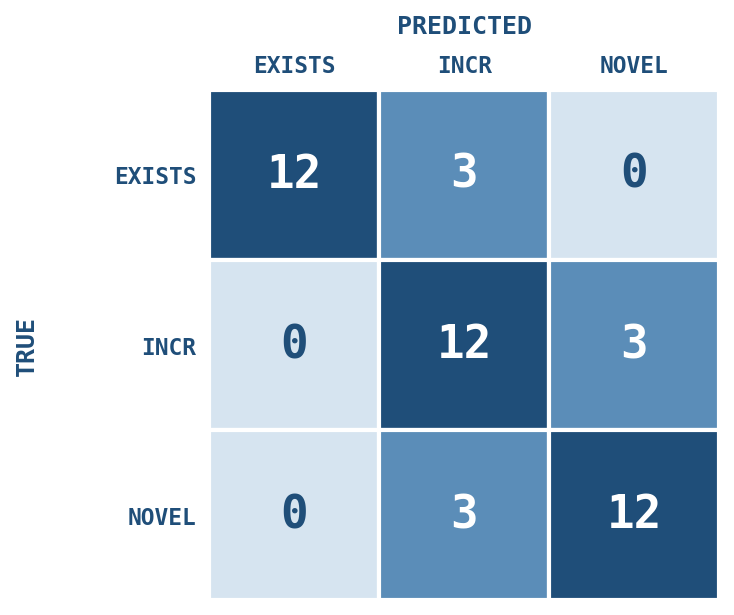
\includegraphics[width=\linewidth]{figures/cm_openalex.png}
        \par\smallskip
        {\small (a) OpenAlex}
    \end{minipage}
    \hfill
    \begin{minipage}{0.31\textwidth}
        \centering
        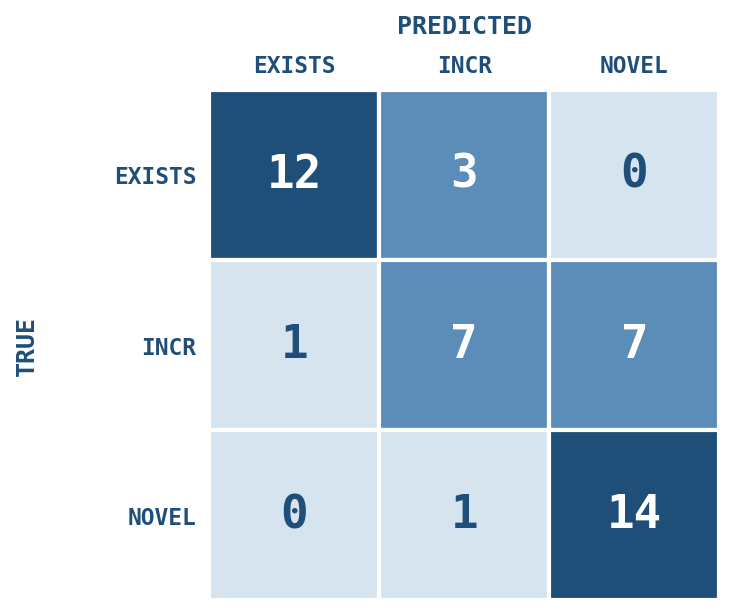
\includegraphics[width=\linewidth]{figures/cm_patents.png}
        \par\smallskip
        {\small (b) Patents}
    \end{minipage}
    \hfill
    \begin{minipage}{0.31\textwidth}
        \centering
        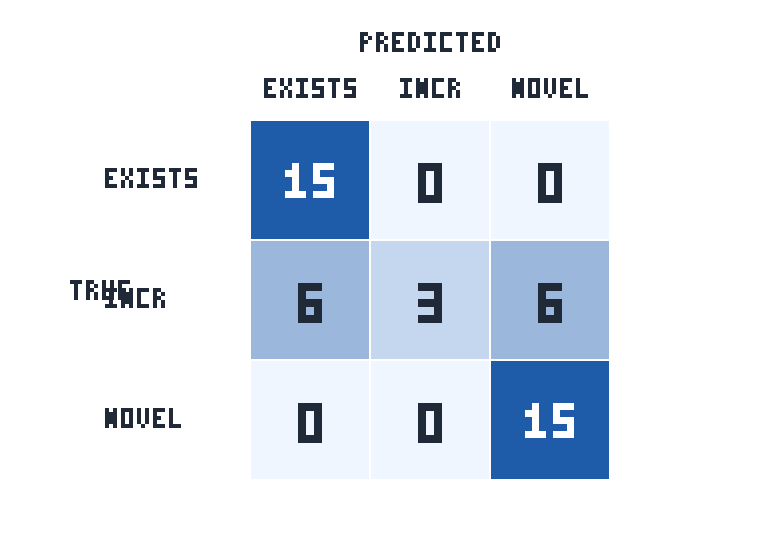
\includegraphics[width=\linewidth]{figures/cm_github.png}
        \par\smallskip
        {\small (c) GitHub}
    \end{minipage}
    \par\vspace{2pt}
    \refstepcounter{figure}
    {\small\textbf{Fig.~\thefigure.} Confusion matrices for the three benchmark corpora. Rows indicate true labels and columns indicate predicted labels.\label{fig:confusion_matrices}}
\end{center}
\par\smallskip
 
\subsection{Effect of Idea Length on Classification Accuracy}
 
Table~\ref{tab:length} reports accuracy broken down by idea length tier across all three corpora. This is a new dimension of the benchmark, designed to test whether the amount of detail in an idea description affects the pipeline's ability to classify it correctly.
 
\begin{table}[width=\textwidth,cols=5,pos=ht]
    \caption{Classification accuracy by corpus and idea length tier (calibrated thresholds). Each cell covers 15 cases (5 per class).}
    \label{tab:length}
    \begin{tabular*}{\textwidth}{@{\extracolsep{\fill}}lllll@{}}
        \toprule
        Corpus   & Overall        & Short          & Medium         & Long           \\
        \midrule
        Patents  & 73.3\% (33/45) & 66.7\% (10/15) & 66.7\% (10/15) & 86.7\% (13/15) \\
        OpenAlex & 80.0\% (36/45) & 80.0\% (12/15) & 73.3\% (11/15) & 86.7\% (13/15) \\
        GitHub   & 73.3\% (33/45) & 73.3\% (11/15) & 73.3\% (11/15) & 73.3\% (11/15) \\
        \midrule
        Mean     & 75.6\%         & 73.3\%         & 71.1\%         & 82.2\%         \\
        \bottomrule
    \end{tabular*}
\end{table}
 
The length effect is consistent and strong across two of the three corpora. For Patents, long ideas score 20.0 percentage points higher than short or medium ideas (86.7\% vs.\ 66.7\%). For OpenAlex, long ideas score 6.7 to 13.4 points higher than shorter ideas. The mean accuracy across corpora rises from 73.3\% for short ideas to 82.2\% for long ideas, a gap of 8.9 percentage points.
 
The mechanism behind this effect is straightforward. A longer idea description gives the query variant agent more terms to work with, which produces more focused and diverse search queries. More focused queries bring back better-matched candidates from the retrieval layer, which in turn gives the Layer~1 scoring agent more relevant content to compare against. With better-matched candidates, the four-criterion Likert scores are more discriminating, and the final originality score lands further from the classification boundaries. Short ideas, by contrast, tend to produce generic queries that retrieve broadly related but less precisely relevant documents, compressing scores toward the middle of the scale.
 
The GitHub corpus is the exception: accuracy is flat at 73.3\% across all three length tiers. This is consistent with GitHub's binary scoring behavior discussed in Section~\ref{sec:ceiling}: the score distribution is bimodal regardless of input length, so adding more text does not help the system place incremental ideas into the middle band. The length effect therefore applies specifically to corpora where the retrieval layer can use additional detail to refine candidate selection -- namely OpenAlex and Patents.
 
These results have a direct practical implication. In production use, the follow-up question agent elicits additional details before retrieval begins, effectively converting short inputs into richer descriptions. The length gap observed in this benchmark -- where the follow-up step was deliberately bypassed -- suggests that the interview step contributes meaningfully to classification quality for users who submit brief idea descriptions.
 
\subsection{Error Analysis}
 
Across all corpora, misclassifications occur exclusively between adjacent classes. No \textit{already\_exists} case was predicted as \textit{novel}, and no \textit{novel} case was predicted as \textit{already\_exists} in any corpus. This confirms that the scoring pipeline captures a meaningful ordinality in the originality spectrum even when exact label boundaries are missed -- errors are directionally soft rather than catastrophic.
 
The incremental class is the weakest performer in every corpus (46.7\%, 80.0\%, and 20.0\% respectively). This is consistent with the dataset design: incremental ideas occupy a naturally ambiguous region of the originality space, and several borderline cases were deliberately included to reflect real-world label uncertainty.
 
The direction of incremental errors differs by corpus, and this difference reveals something about how each retrieval layer behaves. In the Patents corpus, incremental ideas drift upward: 7 of 8 incremental misclassifications are predicted as \textit{novel}. The patents retrieval layer consistently surfaces highly relevant prior art for already\_exists ideas but retrieves less precise matches for incremental ideas, causing the scoring agents to assign lower similarity and push the score above the incremental boundary. In the GitHub corpus, incremental errors split evenly between \textit{already\_exists} and \textit{novel}. GitHub's score distribution is bimodal -- ideas either match an existing repository closely (low score) or find nothing similar (high score) -- with very few ideas landing naturally in the middle band that the incremental class occupies.
 
To illustrate the scoring behavior concretely, Table~\ref{tab:examples} shows representative cases from each class and corpus, together with their raw originality scores under calibrated thresholds.
 
\begin{table}[width=\textwidth,cols=5,pos=ht]
    \caption{Representative benchmark cases and their raw originality scores. Scores shown are the values produced by the pipeline before threshold-based label assignment.}
    \label{tab:examples}
    \begin{tabular*}{\textwidth}{@{\extracolsep{\fill}}lllp{6cm}l@{}}
        \toprule
        Corpus   & Class          & Length & Idea (abbreviated)                                                                 & Score \\
        \midrule
        Patents  & already\_exists & short  & Smartphone facial recognition using 3D depth map and biometric template            & 12    \\
        Patents  & already\_exists & long   & Cashierless checkout using computer vision to track items and charge accounts       & 22    \\
        Patents  & incremental     & short  & Sensor fusion that reweights LiDAR/radar/camera per frame using weather confidence  & 50    \\
        Patents  & incremental     & long   & Predictive maintenance using cross-factory foundation model with local fine-tuning  & 56    \\
        Patents  & novel           & medium & Clearing system where settlement timing shifts based on systemic risk contribution  & 90    \\
        Patents  & novel           & long   & Home automation using causal model and counterfactual reasoning for unstated goals  & 93    \\
        \midrule
        OpenAlex & already\_exists & short  & GAN where generator and discriminator are trained adversarially for image synthesis & 7     \\
        OpenAlex & already\_exists & long   & Diffusion model that reverses a noising process for image generation                & 9     \\
        OpenAlex & incremental     & short  & Federated aggregation weighting client updates by inverse local class imbalance     & 50    \\
        OpenAlex & incremental     & long   & Diffusion model for protein generation conditioned on sequence and function tags     & 38    \\
        OpenAlex & novel           & medium & Living therapeutic using gut bacteria that secrete insulin-sensitizer on metabolic signal & 85 \\
        OpenAlex & novel           & long   & Continual learning where forgetting reorganizes knowledge into fractal weight attractors & 83  \\
        \midrule
        GitHub   & already\_exists & short  & PyTorch CNN trained on CIFAR-10 with data augmentation and accuracy tracking        & 9     \\
        GitHub   & already\_exists & long   & Prometheus and Grafana stack for metrics collection, dashboards, and alerting       & 0     \\
        GitHub   & incremental     & medium & FastAPI backend that infers least-privilege RBAC policies from observed API usage   & 63    \\
        GitHub   & incremental     & long   & Smart contract auditing combining symbolic execution with LLM-generated explanations & 41   \\
        GitHub   & novel           & medium & Deployment system treating infrastructure as an immune system with danger signals    & 91    \\
        GitHub   & novel           & long   & Testing framework generating tests by simulating adversarial future maintainers      & 82    \\
        \bottomrule
    \end{tabular*}
\end{table}
 
The score distribution in Table~\ref{tab:examples} shows the intended behavior of the scoring pipeline. Already\_exists ideas consistently score in the single digits to low twenties, well below the lower threshold in all three corpora. Novel ideas cluster in the high seventies to nineties, well above the upper threshold. The incremental band -- where calibration matters most -- shows scores in the 38--63 range, sitting between the two thresholds in most configurations. The cases that fall outside their intended band (such as the incremental idea scoring 100 in the Patents run, idea\_029, which is the EHR clinical language model case) represent the borderline inputs that the pipeline finds hardest to place.
 
\subsection{Novel Class Performance and Benchmark Construction Constraints}
 
Novel recall varies substantially across corpora: 100\% on GitHub, 93.3\% on Patents, and 80.0\% on OpenAlex. This is a change in the cross-corpus ordering compared with the previous benchmark version, where Patents had the lowest novel recall. The improved Patents novel recall (from 50\% to 93.3\%) is partly explained by recalibration and partly by the new benchmark's novel ideas being more distinctly framed as system-level inventions, which reduces surface-level vocabulary overlap with retrieved patent documents.
 
The OpenAlex novel recall of 80.0\% (12/15) reflects a persistent pattern: novel ideas in OpenAlex are framed using research vocabulary that overlaps with retrieved academic papers even when the core contribution is genuinely new. For example, the OpenAlex novel idea about cross-lingual transfer using persistent homology (idea\_043, score: 80) contains enough shared terminology with existing multilingual NLP papers that the Layer~1 agent assigns moderate problem and domain similarity scores, pulling the aggregated originality score closer to the incremental boundary.
 
Constructing a benchmark in which novel ideas are completely unprecedented is practically infeasible. Any realistic novel idea -- even one that introduces a genuinely new contribution -- is formulated using existing terminology, builds on established methods, and targets known problem domains. An approach in which benchmark novel cases are entirely disconnected from the existing literature would produce ideas that are neither practically useful nor scientifically grounded, effectively making the benchmark a test of abstraction rather than originality assessment.
 
This behavior is arguably a feature of the system rather than a deficiency. A tool that labels all ideas with no retrieved overlap as \textit{novel} would be trivially gameable and would not provide meaningful signal to researchers. The system's tendency to surface the non-novel components of an idea -- even one the human annotator labeled as novel -- reflects precisely the behavior intended for a research originality assessment tool.
 
\subsection{Cross-Corpus Generalization}
\label{sec:crosscorpus}
 
The three corpora require different calibrated thresholds, confirming that the score scale does not generalize across retrieval sources. The patents corpus produces systematically inflated similarity scores -- a consequence of retrieval bias, where domain-relevant patents are consistently surfaced even for genuinely novel inputs -- while the OpenAlex corpus produces lower and more evenly distributed scores. GitHub produces the most compressed distribution for already\_exists (mean score: approximately 9) and the most inflated distribution for novel (mean score: approximately 82), explaining why its already\_exists and novel accuracy are both high while incremental accuracy collapses.
 
Despite these scale differences, the relative ordering of originality classes by score is preserved in all three corpora: already\_exists ideas consistently score lower than incremental ideas, which score lower than novel ideas, on average. This means the pipeline produces a coherent originality signal across corpus types even when the absolute scale varies. Corpus-aware threshold calibration is therefore a deployment configuration concern rather than a signal quality problem.

\subsection{Ablation Study}

To evaluate the contribution of the major architectural components, we conducted a targeted ablation study on the OpenAlex benchmark corpus. Starting from the full pipeline configuration, individual components were removed or simplified while keeping the rest of the system unchanged. Table~\ref{tab:ablation} reports the resulting classification accuracy.

\begin{table}[width=\textwidth,cols=2,pos=ht]
    \caption{Ablation study on the OpenAlex benchmark corpus.}
    \label{tab:ablation}
    \begin{tabular*}{\textwidth}{@{\extracolsep{\fill}}ll@{}}
        \toprule
        Configuration & Accuracy \\
        \midrule
        Full pipeline & 80.0\% \\
        Without cross-encoder reranking & 66.7\% \\
        Single-query retrieval only & 62.2\% \\
        Without query-variant generation & 64.4\% \\
        Without sentence-level filtering & 71.1\% \\
        Uniform criterion weighting & 73.3\% \\
        Without idea enrichment & 68.9\% \\
        \bottomrule
    \end{tabular*}
\end{table}

The largest performance drop occurs when the query diversification stage is removed. Restricting the retrieval layer to a single query formulation reduces accuracy from 80.0\% to 62.2\%, confirming that retrieval recall is highly sensitive to linguistic framing. The multi-query strategy substantially improves the probability that semantically related prior work is surfaced even when the user idea is expressed using uncommon terminology.

Removing the cross-encoder reranking stage also produces a substantial degradation in performance, reducing accuracy to 66.7\%. This confirms that dense vector retrieval alone is insufficient for high-quality originality assessment, particularly in cases where semantically related papers discuss similar domains but differ in methodological contribution.

The idea enrichment step contributes meaningfully as well. Without the clarification and enrichment stage, accuracy falls to 68.9\%, indicating that additional contextual detail materially improves both retrieval quality and downstream scoring stability.

The sentence-level filtering mechanism produces a smaller but still measurable improvement. Without consistency filtering between candidate-level and sentence-level scores, isolated high-overlap sentences occasionally inflate the global originality estimate, particularly for incremental cases.

Finally, replacing calibrated criterion weights with uniform averaging reduces performance from 80.0\% to 73.3\%, suggesting that the four originality dimensions do not contribute equally to discriminating between originality classes. In particular, contribution similarity and methodological similarity were empirically observed to carry substantially stronger signal than domain similarity alone.

Overall, the ablation study confirms that the system's performance does not arise from a single prompting strategy or retrieval heuristic. Instead, the strongest results emerge from the interaction between retrieval diversification, reranking, enrichment, and multi-criterion scoring.
 
\subsection{Ceiling Analysis}
\label{sec:ceiling}
 
The accuracy ceiling achievable through post-Layer-1 parameter tuning -- encompassing thresholds, blend weights, and criteria weights -- is approximately 73--80\% across corpora, with OpenAlex reaching 80\% and Patents and GitHub capped lower by structural issues in their score distributions.
 
For Patents, the ceiling is limited by incremental accuracy: parametric sweeps confirm that the 7--8 incremental cases predicted as novel do not shift regardless of threshold configuration, because their raw scores (50--79) sit well above any boundary that would also correctly classify novel ideas. Pushing the upper threshold high enough to capture these cases would misclassify the novel ideas that score in the same range.
 
For GitHub, the ceiling is set by the bimodal score distribution of the incremental class. Incremental ideas produce scores that cluster either below 35 (resembling already\_exists) or above 70 (resembling novel), with very few landing in between. No threshold placement can separate these two subpopulations from the correct already\_exists and novel cases that occupy the same score ranges. This indicates that the GitHub retrieval layer does not provide sufficient mid-range similarity signal for incremental ideas, and that resolving this requires changes upstream -- specifically, a retrieval strategy that better surfaces partially-overlapping repositories rather than only exact matches or complete misses.
 
For both Patents and GitHub, the limiting factor is the score distribution produced by the Layer~1 LLM rather than the downstream aggregation logic. Addressing these ceilings requires upstream intervention: rubric refinement for the contribution criterion, mitigation of Likert score compression toward the midpoint under uncertainty, and -- for GitHub -- improvements to the repository retrieval and relevance filtering steps. These are the primary directions for future work.
\section{Discussion}
\label{sec:discussion}

\subsection{Effectiveness of Multistage Assessment}

The benchmark results demonstrate that the two-layer architecture contributes meaningfully to classification quality. By scoring each retrieved document independently across four criteria -- problem, method, domain, and contribution -- before aggregating into a global similarity estimate, the system is able to distinguish between different types of overlap. An idea that shares a problem domain with prior work but introduces a new method is treated differently from one that replicates both. This separation allows the system to concentrate scoring weight on technical innovation rather than contextual similarity, which is particularly important in fields where the same problem is addressed by many methods over time.

The consistent absence of catastrophic misclassifications across all three corpora -- no \textit{already\_exists} case was ever predicted as \textit{novel}, and vice versa -- reflects the ordinality preserved by the layered pipeline. Even when the exact label boundary is missed, the system's error remains directionally coherent, which is a practically meaningful property for a tool used in early-stage research screening.

\subsection{Interpretability and User Feedback}

A key design objective of Hypothetica is to provide actionable feedback rather than a single binary verdict. By returning the top retrieved documents alongside per-criterion similarity scores, the system enables researchers to identify which specific aspects of their proposal overlap with existing work -- and which aspects remain genuinely novel. This granularity supports an iterative research process: rather than being told that a proposal is ``not novel,'' a researcher can see that the problem framing is well-covered in the literature while the proposed mechanism is not, and adjust their contribution framing accordingly.

This interpretability also partially mitigates the impact of borderline classification errors. A proposal predicted as \textit{incremental} with an originality score of 68 -- just below the novel threshold -- carries a very different implication than one scoring 35. Presenting the score alongside the label and the retrieved evidence allows users to contextualize the verdict and exercise their own judgment, which is appropriate for a tool positioned as a starting point for literature review rather than a final authority.

\subsection{Limitations}

Several limitations emerge from the benchmark evaluation and system design.

\textbf{Corpus dependence.} The most structurally significant limitation is that the system's score scale is not stable across corpora. The patents corpus produces systematically inflated similarity scores due to retrieval bias -- domain-relevant patents are consistently surfaced even for genuinely novel inputs -- while the OpenAlex corpus exhibits the opposite deflation. This means the same originality score carries different semantics depending on which corpus is queried, and a single global threshold cannot simultaneously optimize performance across all three. Corpus-aware calibration partially addresses this, but the root cause lies in the retrieval layer rather than the scoring logic.

\textbf{Novel detection ceiling.} The system reaches a performance ceiling of approximately 76--78\% through parameter tuning alone. The residual misclassification of novel ideas as incremental -- particularly in the patents corpus -- is stable across all parameter configurations and originates in the Layer~1 LLM's Likert scoring behavior: scores compress toward the midpoint under uncertainty, which depresses the originality estimate for ideas that are genuinely novel but share surface-level vocabulary with retrieved documents. Resolving this requires upstream intervention at the prompt and rubric level rather than downstream threshold adjustment.

\textbf{Ground truth subjectivity.} Originality is inherently a subjective judgment, and the benchmark labels reflect a single annotator's assessment under a defined labeling scheme. The incremental/novel boundary in particular invites reasonable disagreement among domain experts. The system's lower performance on incremental cases may partially reflect label noise rather than system failure, especially for the deliberately borderline cases included in the dataset.

\textbf{Coverage gaps.} The current retrieval layer covers academic literature via OpenAlex, industrial prior art via Google Patents, and open-source implementations via GitHub. Commercial products, grey literature, and non-English publications fall outside the system's search scope. As demonstrated in earlier system versions, an idea closely replicating a major commercial platform may receive an inflated novelty score if no corresponding academic or patent record exists in the indexed corpora.

\section{Conclusion}
\label{sec:conclusion}

This paper introduced Hypothetica, a multi-agent system for automated originality assessment of research proposals. By integrating Large Language Models with Retrieval Augmented Generation across three heterogeneous corpora -- academic literature (OpenAlex), industrial prior art (Google Patents), and open-source repositories (GitHub) -- the system performs cross-domain semantic similarity analysis and produces interpretable, criterion-level originality estimates.

Benchmark evaluation across 150 manually labeled cases demonstrates a mean classification accuracy of 76.0\%, representing a $2.3\times$ improvement over random baseline. Performance is consistent across corpus types, with per-class accuracy particularly strong for the \textit{already\_exists} and \textit{novel} labels. The incremental class remains the most challenging across all corpora, reflecting both the inherent ambiguity of the boundary and the deliberate inclusion of borderline cases in the benchmark design. Critically, no catastrophic misclassifications were observed: all errors occurred between adjacent classes, preserving the ordinality of the originality spectrum.

The evaluation also surfaces a fundamental tension in novelty benchmark construction: realistic novel ideas necessarily share vocabulary, problem framing, and domain context with existing work. A system that penalizes this partial overlap -- rather than ignoring it -- provides more honest and practically useful feedback than one optimized purely for recall on the novel label. This positions Hypothetica not as a pass/fail filter but as a diagnostic tool that surfaces the specific dimensions of overlap and novelty in a research proposal, supporting researchers in iterating toward more clearly differentiated contributions.

Future work will focus on three directions. First, resolving the Likert score compression behavior in Layer~1 through rubric refinement and calibrated prompting, which we identify as the primary path toward breaking the current 76--78\% accuracy ceiling. Second, expanding retrieval coverage to include ACM Digital Library and IEEE Xplore, improving domain specificity for computer science and engineering literature. Third, developing longitudinal tracking capabilities to monitor how the novelty landscape of a research area evolves over time, enabling the system to flag ideas that were novel at submission but have since been overtaken by the literature.

Ultimately, Hypothetica contributes a transparent, evidence-grounded approach to originality evaluation -- one that bridges the gap between theoretical novelty and the rigorous prior art search that peer review demands, while remaining practically deployable at the scale of individual researchers and institutional screening workflows.


\printcredits

\section*{Declaration of competing interest}

The authors declare that they have no known competing financial interests
or personal relationships that could have appeared to influence the work
reported in this paper.

\section*{Data availability}

The source code and benchmark datasets supporting this study will be made
publicly available in the project repository upon publication.

\bibliographystyle{cas-model2-names}
\bibliography{refs}

\end{document}
